%% Packages %%
\documentclass[a4paper, 12pt]{article}  %letter
\usepackage[english]{babel}
\usepackage[utf8]{inputenc}
\usepackage{amsmath}
\usepackage{graphicx}
% \usepackage[colorinlistoftodos]{todonotes}
\usepackage[margin=0.5in]{geometry}
\usepackage[export]{adjustbox}
\usepackage{caption}
\usepackage{subcaption}
\usepackage{wrapfig}
\usepackage{float}
\usepackage{graphics}
\usepackage{tabu}
\usepackage{bm}
\usepackage{lipsum}
\usepackage{physics}
% \usepackage{dcolumn}
% \usepackage{biblatex}
%% End Packages %%
\setlength{\parindent}{0pt}     %manually indent

% \newcommand\blfootnote[1]{% blank footnote
%   \begingroup
%   \renewcommand\thefootnote{}\footnote{#1}%
%   \addtocounter{footnote}{-1}%
%   \endgroup
 

\begin{document}
\title{\textit{Observing nuclear magnetic resonance in aqueous $FeCl_3$ solutions}}
\author{Ruchir Tullu }% Ruchir Tullu (1004220951)
\date{\today}

\maketitle

%%%%%%% Abstract %%%%%%%%
\begin{abstract}
    The NMR characteristics of aqueous $FeCl_3$ solutions were studied using a spectrometer and digital oscilloscope. The longitudinal ($T_1$) and transverse ($T_2$) relation times were found to be 1.02 $\pm$ 0.18 $ms$ and 1.20 $\pm$ 0.23 $ms$, respectively. Two principle values for the gyromagnetic ratio were found, namely $\gamma = 88.12 \pm 4.33 \ MHzT^{-1}$ for a signal frequency of $\sim 5.61 \ MHz$, and $\gamma = 47.12 \pm 2.31 \ MHzT^{-1}$ for a signal frequency of $\sim 3.00 \ MHz$. The corresponding g-factors are $1.84 \pm 0.09$ and $0.98 \pm 0.05$, respectively. The differing values for the gyromagnetic ratio arose from the uncertainty on the signal frequency from the digital oscilloscope.
\end{abstract}
%%%%%%%%%%%% End of Abstract %%%%%%%%%%%%%%%%


%%%%%%% INTRO %%%%%%%%
\section{Introduction}
The following description of nuclear magnetic resonance (NMR) is given in \cite{Lab Manual}:
"Nuclear magnetic resonance is a phenomenon that occurs when photons are resonantly absorbed and emitted by transitions between different energy levels of a nucleus in a magnetic field.". The applications of NMR are numerous, ranging from quantum computing \cite{NMR Quantum Computers-Jones2011, NMR QC-Warren} and medical imaging \cite{ACS NMR} to biotechnology and materials research \cite{Benchtop NMR}.
\newline

The main goal of this experiment was to observe and quantitatively characterize the behaviour of liquid $FeCl_3$ samples in nuclear magnetic resonance by measuring the time constants $T_1$ and $T_2$ as well as the gyromagnetic ratio $\gamma$ of the proton (see Section \ref{Theory} below). We present a broad theoretical overview of NMR, followed by some insight into the experimental methods, and finally the results and interpretations.


%%%%%%%%%%%% End of Intro %%%%%%%%%%%%%%%%



%%%%%%  Relevant Equations and Theory %%%%%%
\subsection{Theory}\label{Theory}
The spin-angular momentum $\Vec{I}$ of a nuclei can be written in terms of the nuclear dipole moment $\Vec{\mu}$ as follows:

\begin{equation}\label{angular momentum}
    \Vec{I} = \Vec{\mu} \cdot \frac{2m}{g q}
\end{equation}

Where the mass and charge are $m$ and $q$ respectively. $g$ is known as the "g-factor"; for a classical rotating object with the same charge and mass distribution, $g = 1$. "For a spin 1/2 quantum point particle, g = 2 (plus small corrections)."\cite{Lab Manual}. The factor of $\frac{2m}{g q}$ is called the gyromagnetic ratio, $\gamma$. When a magnetic dipole is placed in a magnetic field, it can either align itself with or against the magnetic field. For a spin 1/2 particle such as a proton in a magnetic field $\Vec{B} = B_0 \hat{z}$, this leads to the spin-z eigenstates with corresponding energies:

\begin{equation*}\label{spin eigenstates}
\ket{\uparrow_p} \Rightarrow E_{\uparrow} = \frac{1}{2} \gamma \hbar B_0 
\end{equation*}
\begin{equation*}
    \ket{\downarrow_p} \Rightarrow E_{\downarrow} = -\frac{1}{2} \gamma \hbar B_0 
\end{equation*}

"Photons can be resonantly absorbed/emitted when their energy, $h \nu_0$, is equal to the energy difference between the two levels, i.e." \cite{Lab Manual}:

\begin{equation*}
    h \nu_0 = \Delta E = \gamma \hbar B_0
\end{equation*}

The frequency corresponding to this transition is given by $\omega_0 = \nu_0 / 2\pi = \gamma B_0$, and is known as the Larmor frequency. When a spin-1/2 particle in a magnetic field is dressed with pulses at the Larmor frequency, it will induce transitions between the two spin eigenstates. In this experiment, the $FeCl_3$ samples were disturbed by radio frequency pulses known as $\pi$ and $\pi/2$ pulses. $\pi$ pulses correspond to rotating the magnetic moments by $\pi/2$ degrees in the same plane, while $\pi/2$ pulses correspond to rotating the magnetic moments by $\pi$ degrees in the same plane. 
\newline

When studying such resonant systems, two physical quantities interest us, namely $T_1$ and $T_2$. $T_1$ is also called the "spin-lattice"/longitudinal relaxation time, and characterizes how fast a system of spins changes total energy. It is defined as the time taken by a system of magnetic spins to return to thermal equilibrium after being perturbed by a change in the external magnetic field or by a radio frequency pulse. In the former case, if the external magnetic field is suddenly turned on, then the magnetization changes according to  \cite{Lab Manual}: 

\begin{equation*}
    \Vec{M}(t) = \Vec{M}_0 \big ( 1 - e^{-t/T1} \big )
\end{equation*}

If instead a radio frequency pulse is applied, the spin system decays back to it's equilibrium state with time constant $T_1$, producing an observable "free-induction tail" \cite{Lab Manual}. 
\newline

$T_2$ is known as the "spin-spin"/transverse relaxation time, and characterizes how fast spins in a system move out of phase with respect to each other (decay phase coherence) due to "static" internal magnetic inhomogeneities \footnote{There is another time constant $T^*_2$ which characterizes the decay phase coherence when magnetic inhomogeneities are includes, however these are not considered in this experiment \cite{Lab Manual}.}\cite{Lab Manual}. We note in particular that $T_2 \leq T_1$. For non-viscous liquids, $T_1 \approx T_2$ \cite{Lab Manual}. 

\subsection{Methods}\label{Methods}

To measure $T_2$, we use the method of spin-echoes. As described in \cite{Lab Manual}:
"The method of spin-echoes reduces the effect of field inhomogeneities. If a $\pi/2$ is
followed by a $\pi$ pulse applied at a time $\tau$ later, the $\pi$ pulse will flip the spins so they start precessing in the opposite direction. Quickly precessing nuclei now find themselves behind the slowly precessing nuclei, but they catch up so that an additional time $\tau$ later all the nuclei will come back into phase and produce a signal in the detector coil. This is a spin-echo. The loss in
amplitude of the signal is due solely to any irreversible process and will occur at the time rate $T_2$. Repeated $\pi/2$, $\pi$ pulses with different delay times $\tau$ can thus be used to measure $T_2$." This effect is illustrated in Figure \ref{fig:spin_echo}. The height of the spin echo decays exponentially, and can be measured to find $T_2$:

\begin{equation}\label{T2}
    I^{rf} = I_0^{rf} e^{-t/T_2}
\end{equation}


To measure $T_1$, we use the method of the inversion recovery($\pi$-$\pi/2$) sequence. After being disturbed by a $\pi$ pulse, the magnetization evolves according to \cite{Lab Manual}:

\begin{equation}\label{T1}
    M(t) = M_0 \big ( 1 - 2 e^{-t/T_1} \big )
\end{equation}

Here, $M(t)$ corresponds to the height of the induction tail of the second pulse \cite{Lab Manual}. Thus, by measuring the height of the induction tail for various delay times, one can determine $T_1$.



\begin{figure}[htb]
    \centering
    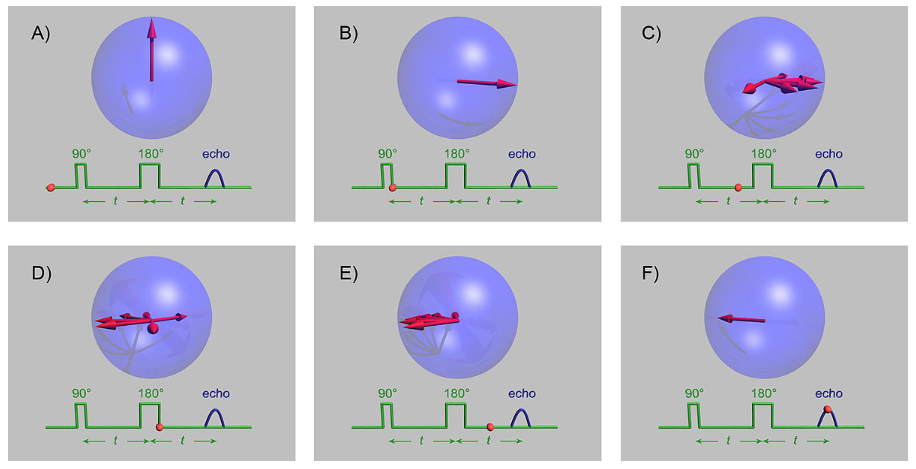
\includegraphics[width = \textwidth]{spin_echoes.PNG}
    \caption{Illustration of the method of spin-echoes. In (A) the spin system is in the spin-up state, which gets flipped to the x-y plane when a $\pi/2$ pulse is applied in (B). The spins begin to precess at different rates due to local magnetic field inhomegeneities (C). A $\pi$ pulse is then applied in (D), such that the spins flip by $\pi$ radians. The spins then begin to realign (E), and at some time later, the spins are all re-aligned (F), corresponding to an observable spin-echo signal. Figure taken from \cite{Spin Echo}.}
    \label{fig:spin_echo}
\end{figure}



%%%%% End of Relevant Equations and Theory %%%%

%%%%%%%%%%%%%%%%%% Apparatus %%%%%%%%%%%%%%%%%%%%
\section{Apparatus}
% A spectrometer was used in addition to a digital oscilloscope for the purposes of measurement.

 A probe coil (containing the liquid $FeCl_3$ sample to be analyzed) connected to a spectrometer was inserted into the field generated by a large electromagnet powered separately by a DC power source. A schematic of the spectrometer and probe can be seen in Figure \ref{fig:schematic}. The radio frequency pulses were generated and detected by the spectrometer, while an oscilloscope was used to check the validity of the signals. The precise design of the spectrometer ensured that voltages greater than $\sim 0.6 \ V$ appeared at the sample in the coil, thereby preventing low-voltage noise \cite{Lab Manual}. The operating range of the DC power source was on the order of $10 \ V$, $10^0 \ A$ \footnote{Typical currents used were around 5-6 $A$ and did not exceed 7 $A$, and typical voltages were around 40 $V$.}. The power source was operated in the voltage limiting mode for the mode accurate current and voltage readings. Lastly, the measurement of the magnetic field inside the electromagnet was taken using a Bell 620 Gaussmeter, which was calibrated using a standard magnet with a known magnetic field. This yielded a magnetic field strength of $0.4 \pm 0.02 T$ generated by the electromagnet. 
 
 \begin{figure}[htb]
     \centering
     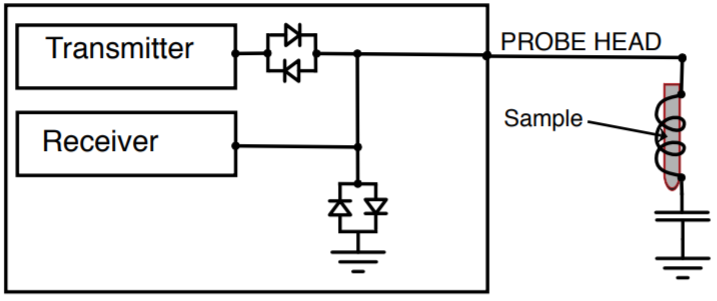
\includegraphics[scale=0.75]{schematic.PNG}
     \caption{Schematic of the experimental setup (taken from \cite{Lab Manual}).}
     \label{fig:schematic}
 \end{figure}

%%%%%%%%%%%%%%%% End of Apparatus %%%%%%%%%%%%%%%%%%



%%%%% Experimental Setup and Procedure %%%%
% \subsection{Experimental Setup and Procedure}

%%%%% End of Experimental Setup and Procedure %%%%


%%%%%%%%%%%% Results and Data Analysis %%%%%%%%%%%%%
\section{Observations \& Results}\label{results}

Data was collected for the height of the spin echo and free induction tails at different delay times between incoming radio frequency pulses to determine $T_1$ and $T_2$. The raw data for these measurements can be seen in Figure \ref{fig:raw_data}. The observed shape is what we expect based on Equations \ref{T2}, \ref{T1}; we will verify that these fits are indeed exponential in nature. Figure \ref{ODR fits} shows the orthogonal distance regression fits \footnote{Code used to analyze the data is available at \cite{ODR}.} for the data in Figure \ref{fig:raw_data}. The following table summarizes the parameters obtained from the fit:

\begin{table}[htb]
    \centering
    \begin{tabular}{|c|c|c|}
    \hline
         & $T_1$ (Figure \ref{fig:f1}) & $T_2$ (Figure \ref{fig:f1})\\
        \hline
        $\chi^2$ CDF & 0.76\% & 67.20\% \\
        
        $\chi^2 / dof$ & 3.48 & 0.51  \\
        
        Decay constant ($\pm$ ms) & 1.02 $\pm$ 0.18 & 1.20 $\pm$ 0.23          \\
        \hline
    \end{tabular}
    \caption{Fitting parameters for the orthogonal regression fits for Figure \ref{fig:raw_data}}
    \label{tab:fit_parameters}
\end{table}


\begin{figure}[htb]
    \centering
    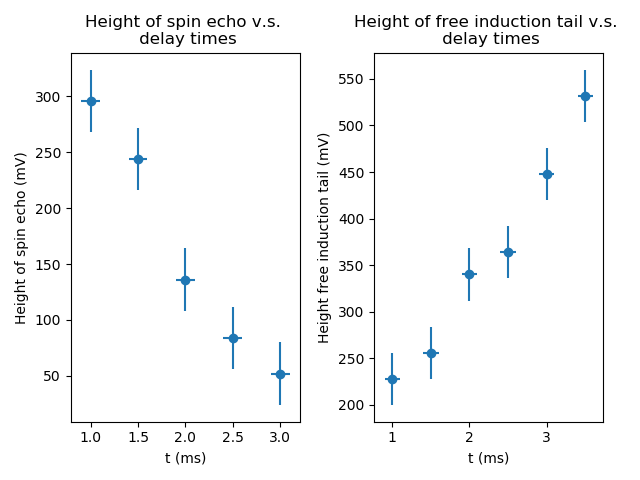
\includegraphics[scale=0.65]{raw_data.png}
    \caption{Heights of spin echo and free induction tail signals for $T_2$ and $T_1$ measurements respectively, measured in a magnetic field strength of $0.4 \pm 0.02 T$}
    \label{fig:raw_data}
\end{figure}


\begin{figure}[!tbp]
  \begin{subfigure}[b]{0.5\textwidth}
    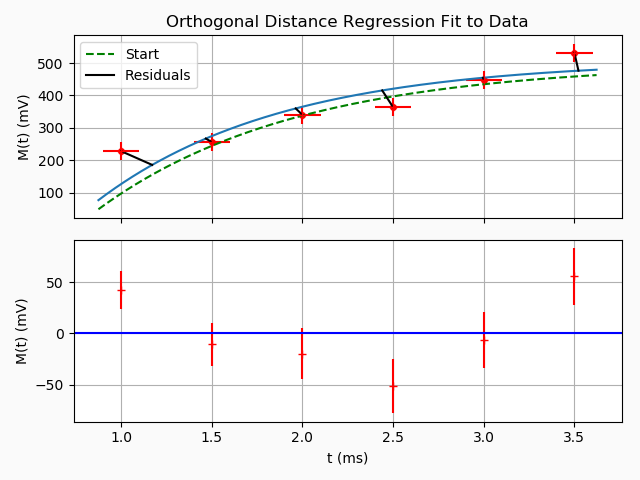
\includegraphics[width=\textwidth]{T1.png}
    \caption{Height of free induction tail plotted against different delay times to determine $T_1$}
    \label{fig:f1}
  \end{subfigure}
  \hfill
  \begin{subfigure}[b]{0.5\textwidth}
    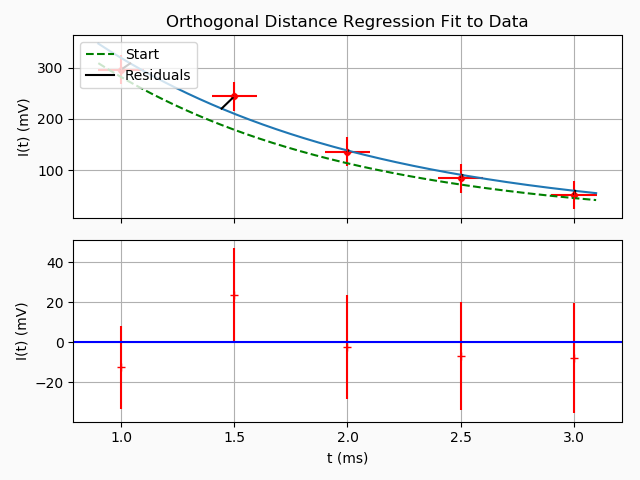
\includegraphics[width=\textwidth]{T2.png}
    \caption{Height of spin echo plotted against different delay times to determine $T_2$}
    \label{fig:f2}
  \end{subfigure}
  \caption{Orthogonal distance regression fits for determining $T_1$ and $T_2$}
\label{ODR fits}
\end{figure}
 
 Two values for the gyromagnetic ratio were found; there were 2 distinct frequencies observed on the oscilloscope when observing the NMR signal from the spectrometer. These arose when viewing the signal at different time scales on the oscilloscope. For a frequency of $\sim 5.61 \ MHz$, we obtain $\gamma = 88.12 \pm 4.33 \ MHzT^{-1}$; for a frequency of $\sim 3 \ MHz$, we obtain $\gamma = 47.12 \pm 2.31 \ MHzT^{-1}$. The corresponding g-factors are $1.84 \pm 0.09$ and $0.98 \pm 0.05$, respectively. Section \ref{Discussion} discusses some reasons behind the different frequencies, and how the exact frequency could have been better determined.
 
 
 
%%%%%%%%%%%% End of Results and Data Analysis %%%%%%%%%%%%%


%%%%%%%%%%% Discussion Start %%%%%%%%%%%%
\section{Discussion and Results}\label{Discussion}
As can be seen in Table \ref{tab:fit_parameters}, we see that $T_1 < T_2$ for the $FeCl_3$ solution. However, $T_1$ and $T_2$ fall within range of each other's uncertainties, and so the property that $T_1 \approx T_2$ for non-viscous liquids may indeed hold here. The $T_2$ fit has a reasonable $\chi^2 / dof$ and $\chi^2$ CDF, however the same cannot be said for the $T_1$ fit. The large values of $\chi^2 / dof$ and $\chi^2$ CDF indicate here that the fit is not good, and that the uncertainties were under-estimated. However, since the uncertainty estimates for $T_2$ were the same as for $T_1$, and they yielded a reasonable $\chi^2 / dof$ and $\chi^2$ CDF, it is safe to say that the large values for these parameters in the $T_1$ fits are a result of the relatively skewed data points as seen in Figure \ref{fig:f1}. By observation, the data points are not oriented exactly as per an exponential fit, with some points being skewed, and hence result in a bad fit for $T_1$. Increased data collection could resulted in a more reasonable fit.
\newline

The different values for the frequency of the NMR signal lead to two different values for the gyromagnetic ratio of the proton (see Section \ref{results}). According to \cite{Gyromagnetic_ratio_NIST}, $\gamma =  42.57608(12) \ MHz T^{-1}$, which is similar to one of the values obtained. However, for this value obtained we find that $g \sim 1$, which is not what we expect for a quantum point particle with spin 1/2. The other result obtained yields a $g$-value much closer to 2 for a much different frequency. The apparent disagreement in the results for $g$ may also be explained by aliasing effects present in the oscilloscope; that is, an incorrect sampling frequency may have lead to erroneous frequencies of the incoming signal being recorded (see \cite{aliasing}). The exact frequency of the signal could have been determined by using a spectrum analyzer to give the dominant frequency in the signal (by means of a Fourier transform), however this step was not done due to time considerations. 
\newline

The major source of uncertainties was systematic; from the imprecision of the settings for the delay times on the spectrometer, as well as the noise on the oscilloscope signal. Reduction of these uncertainties would result in more accurate results. Statistical uncertainties could also be reduced by taking more trials.



% \subsection{Experimental Errors}
% We may now consider some sources of error which may have affected the results of the experiment either through random or systematic error. Some potential sources of error are as follows:

% \begin{itemize}
%     \item 
    
% \end{itemize}

%%%%%%%%%%%%% Discussion Ends %%%%%%%%%%%%%


%%%%%%%%%%%%% Conclusion %%%%%%%%%%%%%%
\section{Conclusions and Outlook}
In this experiment we studied the NMR characteristics of aqueous $FeCl_3$ solutions. The longitudinal ($T_1$) and transverse ($T_2$) relation times were found to be 1.02 $\pm$ 0.18 $ms$ and 1.20 $\pm$ 0.23 $ms$, respectively. These values satisfy the property that $T_1 \approx T_2$ for non-viscous liquids. Two principle values for the gyromagnetic ratio were found, namely $\gamma = 88.12 \pm 4.33 \ MHzT^{-1}$ for a signal frequency of $\sim 5.61 \ MHz$, and $\gamma = 47.12 \pm 2.31 \ MHzT^{-1}$ for a signal frequency of $\sim 3.00 \ MHz$. The corresponding g-factors are $1.84 \pm 0.09$ and $0.98 \pm 0.05$, respectively. We expect that $g = 2$ for a quantum point particle with spin 1/2; however, we also expect that the gyromagnetic ratio has a value of $42.57608(12) \ MHz T^{-1}$ \cite{Gyromagnetic_ratio_NIST}. The seemingly contradicting results obtained experimentally can be resolved in the future by using a spectrum analyzer to precisely determine the dominant frequency of the NMR signal (which could also prevent aliasing effects), which in turn determines the gyromagnetic ratio.

%%%%%%%%%%%% End of Conclusion %%%%%%%%%%%%%

% \newpage
%%%%%%%%%%%%%%% References %%%%%%%%%%%%%%%%%%%
\begin{thebibliography}{9}

\bibitem{Lab Manual}
D. Bailey, J. Harlow, J. Vise, J. Pitre, NMR Nuclear Magnetic Resonance, University of Toronto, 1988. https://www.physics.utoronto.ca/~phy326/nmr/nmr.pdf (accessed October, 2019).

\bibitem{Spin Echo}
Gavin W Morley, SpinEcho GWM stills.jpg,     Wikimedia Commons. (2011). https://commons.wikimedia.org/wiki/File:SpinEcho\_GWM\_stills.jpg (accessed October, 2019).

\bibitem{ODR}
D. Bailey, odr\_fit\_to\_data.py, (2013). https://www.physics.utoronto.ca/~phy326/python/\\odr\_fit\_to\_data.py (accessed October, 2019).

\bibitem{Gyromagnetic_ratio_NIST}
P. Keller, Values of Gyromagnetic Ratios, 2017. https://www.metrolab.com/wp-content/uploads/2017/03/Values-of-Gyromagnetic-Ratios.pdf (accessed October, 2019).

\bibitem{Benchtop NMR}
Nanalysis Corp., Applications — Benchtop NMR, Nanalysis. (n.d.). https://www.nanalysis.com/applications (accessed November, 2019).

\bibitem{NMR Quantum Computers-Jones2011}
J.A. Jones, Quantum computing with NMR, Progress in Nuclear Magnetic Resonance Spectroscopy. 59 (2011) 91–120. doi:10.1016/j.pnmrs.2010.11.001.(accessed November, 2019).

\bibitem{NMR QC-Warren}
W.S. Warren;, The Usefulness of NMR Quantum Computing, 277 (1997) 1688–1690. doi:10.1126/science.277.5332.1688. (accessed November, 2019).

\bibitem{ACS NMR}
American Chemical Society, NMR and MRI: Applications in Chemistry and Medicine, American Chemical Society. (2011). https://www.acs.org/content/acs/en/education/whatischemistry/landmarks/mri.html\ (accessed November, 2019).

\bibitem{aliasing}
H. Gonçalves, Aliasing, OnMyPhD. (n.d.). \\ http://www.onmyphd.com/?p=aliasing\#h2\_samplingtheorem (accessed November, 2019).

\end{thebibliography}

%%%%%%%%%%%%%% End of References %%%%%%%%%%%%%%%%%%

\end{document}

%%%%%%%%%%%%%%%% Finish %%%%%%%%%%%%%%%%%
